\let\negmedspace\undefined
\let\negthickspace\undefined
\documentclass[journal,12pt,onecolumn]{IEEEtran}
\usepackage{cite}
\usepackage{amsmath,amssymb,amsfonts,amsthm}
\usepackage{algorithmic}
\usepackage{graphicx}
\usepackage{textcomp}
\usepackage{xcolor}
\usepackage{txfonts}
\usepackage{listings}
\usepackage{enumitem}
\usepackage{mathtools}
\usepackage{gensymb}
\usepackage{comment}
\usepackage[breaklinks=true]{hyperref}
\usepackage{tkz-euclide} % loads  TikZ and tkz-base
\usepackage{listings}
\usepackage[latin1]{inputenc}                                
\usepackage{color}                                            
\usepackage{array}                                            
\usepackage{longtable}                                       
\usepackage{calc}                                             
\usepackage{multirow}                                         
\usepackage{hhline}                                           
\usepackage{ifthen}                                           
\usepackage{lscape}
\usepackage{caption}
\usepackage{subcaption}
\usepackage{float}


\newtheorem{theorem}{Theorem}[section]
\newtheorem{problem}{Problem}
\newtheorem{proposition}{Proposition}[section]
\newtheorem{lemma}{Lemma}[section]
\newtheorem{corollary}[theorem]{Corollary}
\newtheorem{example}{Example}[section]
\newtheorem{definition}[problem]{Definition}
%\newtheorem{thm}{Theorem}[section] 
%\newtheorem{defn}[thm]{Definition}
%\newtheorem{algorithm}{Algorithm}[section]
%\newtheorem{cor}{Corollary}
\newcommand{\BEQA}{\begin{eqnarray}}
\newcommand{\EEQA}{\end{eqnarray}}
\newcommand{\define}{\stackrel{\triangle}{=}}
\theoremstyle{remark}
\newtheorem{rem}{Remark}
%\bibliographystyle{ieeetr}

\begin{document}

%
\providecommand{\pr}[1]{\ensuremath{\Pr\left(#1\right)}}
\providecommand{\prt}[2]{\ensuremath{p_{#1}^{\left(#2\right)} }}        % own macro for this question
\providecommand{\qfunc}[1]{\ensuremath{Q\left(#1\right)}}
\providecommand{\sbrak}[1]{\ensuremath{{}\left[#1\right]}}
\providecommand{\lsbrak}[1]{\ensuremath{{}\left[#1\right.}}
\providecommand{\rsbrak}[1]{\ensuremath{{}\left.#1\right]}}
\providecommand{\brak}[1]{\ensuremath{\left(#1\right)}}
\providecommand{\lbrak}[1]{\ensuremath{\left(#1\right.}}
\providecommand{\rbrak}[1]{\ensuremath{\left.#1\right)}}
\providecommand{\cbrak}[1]{\ensuremath{\left\{#1\right\}}}
\providecommand{\lcbrak}[1]{\ensuremath{\left\{#1\right.}}
\providecommand{\rcbrak}[1]{\ensuremath{\left.#1\right\}}}
\newcommand{\sgn}{\mathop{\mathrm{sgn}}}
\providecommand{\abs}[1]{\left\vert#1\right\vert}
\providecommand{\res}[1]{\Res\displaylimits_{#1}} 
\providecommand{\norm}[1]{\left\lVert#1\right\rVert}
%\providecommand{\norm}[1]{\lVert#1\rVert}
\providecommand{\mtx}[1]{\mathbf{#1}}
\providecommand{\mean}[1]{E\left[ #1 \right]}
\providecommand{\cond}[2]{#1\middle|#2}
\providecommand{\fourier}{\overset{\mathcal{F}}{ \rightleftharpoons}}
\newenvironment{amatrix}[1]{%
  \left(\begin{array}{@{}*{#1}{c}|c@{}}
}{%
  \end{array}\right)
}
%\providecommand{\hilbert}{\overset{\mathcal{H}}{ \rightleftharpoons}}
%\providecommand{\system}{\overset{\mathcal{H}}{ \longleftrightarrow}}
        %\newcommand{\solution}[2]{\textbf{Solution:}{#1}}
\newcommand{\solution}{\noindent \textbf{Solution: }}
\newcommand{\cosec}{\,\text{cosec}\,}
\providecommand{\dec}[2]{\ensuremath{\overset{#1}{\underset{#2}{\gtrless}}}}
\newcommand{\myvec}[1]{\ensuremath{\begin{pmatrix}#1\end{pmatrix}}}
\newcommand{\mydet}[1]{\ensuremath{\begin{vmatrix}#1\end{vmatrix}}}
\newcommand{\myaugvec}[2]{\ensuremath{\begin{amatrix}{#1}#2\end{amatrix}}}
\providecommand{\rank}{\text{rank}}
\providecommand{\pr}[1]{\ensuremath{\Pr\left(#1\right)}}
\providecommand{\qfunc}[1]{\ensuremath{Q\left(#1\right)}}
        \newcommand*{\permcomb}[4][0mu]{{{}^{#3}\mkern#1#2_{#4}}}
\newcommand*{\perm}[1][-3mu]{\permcomb[#1]{P}}
\newcommand*{\comb}[1][-1mu]{\permcomb[#1]{C}}
\providecommand{\qfunc}[1]{\ensuremath{Q\left(#1\right)}}
\providecommand{\gauss}[2]{\mathcal{N}\ensuremath{\left(#1,#2\right)}}
\providecommand{\diff}[2]{\ensuremath{\frac{d{#1}}{d{#2}}}}
\providecommand{\myceil}[1]{\left \lceil #1 \right \rceil }
\newcommand\figref{Fig.~\ref}
\newcommand\tabref{Table~\ref}
\newcommand{\sinc}{\,\text{sinc}\,}
\newcommand{\rect}{\,\text{rect}\,}
%%
%       %\newcommand{\solution}[2]{\textbf{Solution:}{#1}}
%\newcommand{\solution}{\noindent \textbf{Solution: }}
%\newcommand{\cosec}{\,\text{cosec}\,}
%\numberwithin{equation}{section}
%\numberwithin{equation}{subsection}
%\numberwithin{problem}{section}
%\numberwithin{definition}{section}
%\makeatletter
%\@addtoreset{figure}{problem}
%\makeatother

%\let\StandardTheFigure\thefigure
\let\vec\mathbf

\bibliographystyle{IEEEtran}

\vspace{3cm}
\title{Assignment}
\author{EE23BTECH11001 - Aashna Sahu}
\maketitle
\bigskip

\renewcommand{\thefigure}{\theenumi}
\renewcommand{\thetable}{\theenumi}
%\renewcommand{\theequation}{\theenumi}
Q:Which one of the options given is the inverse Laplace transform of $\frac{1}{s^3-s}$?\\
$u(t)$ denotes the unit-step function.
\begin{enumerate}[label=(\Alph*)]
\item $\left(-1+\frac{1}{2}e^{-t}+\frac{1}{2}e^t\right)u(t)$\\
\item $\left(\frac{1}{3}e^{-t}-e^t\right)u(t)$\\
\item $\left(-1+\frac{1}{2}e^{-(t-1)}+\frac{1}{2}e^{(t-1)}\right)u(t-1)$\\
\item $\left(-1-\frac{1}{2}e^{-(t-1)}-\frac{1}{2}e^{(t-1)}\right)u(t-1)$\\
\end{enumerate}
\hfill(GATE ME 2023)

\solution
\\
Using partial fraction,\\
\begin{align}
\frac{1}{s^3-s}=\frac{A}{s}+\frac{B}{s+1}+\frac{C}{s-1}
\end{align}
On Solving,
\begin{align}
\implies A=-1\quad B=\frac{1}{2} \quad C=\frac{1}{2}\\
X(s)=\frac{-1}{s}+\frac{1}{2(s+1)}+\frac{1}{2(s-1)}\\
\text{As} \quad e^{-at}u(t) \xrightarrow{\mathcal{L}} \frac{1}{s+a}\quad \Re(s)>-a\\
\text{And} \quad -e^{-at}u(-t) \xrightarrow{\mathcal{L}} \frac{1}{s+a}\quad \Re(s)<-a
\end{align}
Now,
\begin{align}
\mathcal{L}^{-1}(X(s))=x(t)
\end{align}

There are 4 cases possible,
\begin{align}
x(t)=
\begin{cases}
        \left(1-\frac{1}{2}e^{-t}-\frac{1}{2}e^t\right)u(-t) & \Re(s)<-1 \\
        \\
        -1u(-t)+\frac{1}{2}e^{-t}u(t)-\frac{1}{2}e^tu(-t) & \Re(s)\in(-1,0)\\
        \\
        -u(t)+\frac{1}{2}e^{-t}u(t)-\frac{1}{2}e^tu(-t) & \Re(s)\in(0,1)\\
        \\
        \left(-1+\frac{1}{2}e^{-t}+\frac{1}{2}e^t\right)u(t) & \Re(s)>1
\end{cases}
\end{align}\\
 
Thus the correct option is (A) $\left(-1+\frac{1}{2}e^{-t}+\frac{1}{2}e^t\right)u(t)$ for $\Re(s)>1$

\begin{figure}[H]
  \centering
  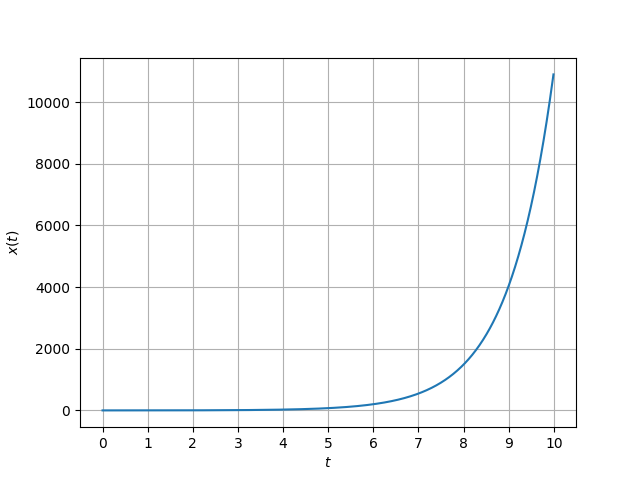
\includegraphics[width=1.0\columnwidth]{figs/plot1.png}
  \caption{Plot for x(t)}
  \label{fig:fig1}
\end{figure}
\end{document}
